\section{Pipeline and Experimental Design}
\label{sec:pipeline-design}
\subsection{The Curation Pipeline and Its Components}
\label{sec:pipeline}

All experiments use one pipeline family, which reads a corpus split into chunks and produces a Web Ontology Language (OWL) style schema (TBox) and a set of facts (ABox) stored as Resource Description Framework (RDF) triples. Formally, a constructed knowledge graph is represented as $G = (V, E)$, where $V$ denotes the set of entity vertices and $E \subseteq V \times \mathcal{R} \times V$ denotes directed relational edges labeled by predicates from a relation vocabulary $\mathcal{R}$. Figure~\ref{fig:pipeline} shows the five stages, and Table~\ref{tab:experiments} lists the studies, Exp1 to Exp8.

\begin{figure*}[t]
\centering
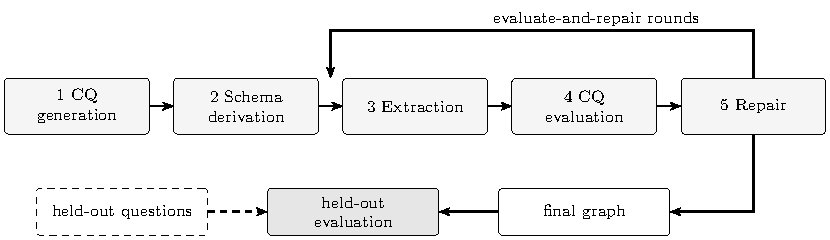
\includegraphics[width=\textwidth]{fig_pipeline.pdf}
\caption{The pipeline builds the graph in five stages, and evaluate-and-repair rounds loop from repair back to schema derivation and extraction. Held-out questions reach only the evaluation of the final graph.}
\label{fig:pipeline}
\end{figure*}

\paragraph{Stages.}
\begin{enumerate}
  \item \emph{CQ generation.} The generator reads a batch of chunks and writes questions that a reader of those chunks should be able to answer. Each CQ, a question generated from a chunk, keeps its source chunk and an expected answer span, which code checks against the chunk.
  \item \emph{Schema derivation.} Classes and properties are derived from the CQs.
  \item \emph{Extraction.} Facts are extracted chunk by chunk, guided by the current schema. Every fact keeps the chunk it came from.
  \item \emph{CQ evaluation.} Each CQ is translated to SPARQL Protocol and RDF Query Language (SPARQL) queries and run against the graph. A deterministic rule first checks that the expected span appears in the result rows. An LLM judge then grades the answer 0, 1 or 2.
  \item \emph{Repair.} Failed CQs are attributed either to the query or to the graph. Graph-side failures produce patches (added facts, merged entities, corrected values or new properties). A gate scores each patch on a reserved set of curation CQs, never on held-out questions, and accepts or rejects it.
\end{enumerate}

\paragraph{Components under test.}
Every study except the Exp6 error analysis changes one of the following components or removes one from the combined pipeline.
\begin{description}
  \item[Relation list.] A relation list from the training split: the 22 most frequent relation types (share of at least 0.1\%) in the evidence inventory of the 2WikiMultihopQA training split, where no evaluation question was used. The names cover the relations of 98.4\% of the 1,216 gold evidence items of the evaluation set. Only the names are given, in alphabetical order, with no frequencies or examples. The names enter the prompts as one block with the same wording and position in every arm with the list (Table~\ref{tab:arms}), and Appendix~\ref{app:seednames} lists them.
  \item[CQ coverage.] Coverage is the share of chunks that are the source of at least one CQ. A first round writes a fixed number of CQs (40 in most experiments). \emph{Expansion} adds CQs over several rounds, each time drawing from chunks that are not yet the source of any CQ, until every chunk is covered.
  \item[CQ count.] Exp8 varies the number of CQs at a fixed or increased token budget.
  \item[Evaluate-and-repair rounds.] Stages 4 and 5 run for several rounds. The loop used in Exp5, and as the LOOP baseline in Exp7, repairs queries first and patches only graph-side failures.
  \item[Budget and extraction passes.] The total number of tokens, and how the remainder is spent. In the combined pipeline, tokens left after expansion go to additional full-corpus extraction passes that ask for facts missing from the current graph.
\end{description}

\paragraph{Where the 22 names come from.}
The original list is the set of relation types with a share of at least 0.1\% in the evidence inventory of the training split, which gives 22 names. An induced list uses no question and no gold relation. The extraction model reads 300 randomly sampled passages (title and first 1,200 characters) in 20 batches of 15 and proposes up to 15 relation names per batch, and the names are normalised to one to four lowercase words. The 80 names proposed in the most batches go to one model call that merges near-duplicates and keeps exactly 22. Induced lists have 22 names so that they equal the size of the original list and differ only in content (Appendix~\ref{app:seednames}).

Table~\ref{tab:arms} defines every arm. The \emph{combined pipeline} (``Combined'' in tables) starts from the relation list, and a \emph{+vocab} suffix on any other arm name means the same pipeline run with that list.

\begin{table*}[t]
\centering
\small\setlength{\tabcolsep}{3.5pt}
\caption{The arms compared. ``Reads and writes'' gives what each arm takes in and produces; the last column gives where the relation list enters the prompts when the arm runs with it.}
\label{tab:arms}
\begin{tabular}{lP{6.2cm}cP{4.6cm}}
\toprule
Arm & Reads and writes & CQs & Where the list enters \\
\midrule
L0 (single pass) & Chunks $\rightarrow$ 40 CQs $\rightarrow$ schema of at most 36 properties $\rightarrow$ facts extracted from every chunk & yes & CQ generation and schema derivation \\
G (Exp4, Exp5) & L0 with the CQ set expanded until every chunk is a CQ source & yes & as L0 \\
GR (Exp4, Exp5) & G plus evaluate-and-repair rounds & yes & as L0 \\
LOOP & L0, then three rounds of CQ evaluation and repair with 20 new CQs per round & yes & CQ generation, schema extension and schema patches \\
Combined & Relation list, CQs expanded to every chunk, an incremental schema with deterministic de-duplication, and extra extraction passes up to the token total of LOOP+vocab on the same unit; CQ evaluation only as an acceptance test, no repair step. ``First pass only'' stops after the first full extraction pass & yes & CQ generation, schema derivation and schema extension \\
U-ext (extraction without CQs) & No CQs and no schema: free-form predicates from every chunk, one call per chunk; the schema is derived afterwards & no & Extraction prompt, after the chunk text and before the instruction (U-ext+vocab) \\
+vocab & Any arm above run with the 22-name relation list (L0+vocab, LOOP+vocab, and U-ext+vocab, called \emph{seeded extraction}; ``Combined'' always has it unless marked no list) & as arm & as in the arm's row \\
L0+vocab$K$ & L0 given $K$ of the 22 names ($K$ = 6, 11, 17; nested random subsets) & yes & CQ generation and schema derivation \\
iText2KG, EDC, AutoSchemaKG & Chunks $\rightarrow$ facts with each public extractor's released defaults and no relation list (EDC also once with the list, Section~\ref{sec:res-cost}); EDC and AutoSchemaKG induce and canonicalise their own schema, and AutoSchemaKG's entity-relation triples are scored & no & none \\
\bottomrule
\end{tabular}
\end{table*}
